\chapter{Implementacja}
\label{sec:implementacja}

\section{Docker}
	Do zbudowania aplikacji użyto narzędzia \emph{docker-compose}.
	Pozwala ono definiować kontenery, które uruchomione zostaną we wspólnym środowisku.
	Dla każdego kontenera zdefiniowane zostały następujące właściwości:
	\begin{description}
		\item[container\_name] nazwa kontenera
		\item[image] obraz, z którego będzie zbudowany
		\item[build] instrukcje do zbudowania obrazu
		\item[networks] wewnętrzne sieci, do których podłączony zostanie kontener
		\item[volumes] foldery hosta, które zostaną zmapowane do adresu wewnątrz kontenera
		\item[ports] porty hosta, które zostaną zmapowane na porty kontenera
		\item[environment] zmienne środowiskowe wewnątrz kontenera
		\item[depends\_on] kontenery, które powinny zostać zbudowane przed opisywanym kontenerem
	\end{description}
	Każdy kontener musi mieć zdefiniowany \textbf{image}, z którego zostanie zbudowany
	lub parametry \textbf{build} z adresem pliku Dockerfile zawierającym przepis na zbudowanie obrazu.
	
	Pliki docker-compose są przyłączeniowe; podczas budowania środowiska można zdefiniować więcej niż jeden.
	Zaletę tę wykorzystano w projekcie i rozdzielono pliki docker-compose na wersje odpowiadające odpowiednim środowiskom.
	Proces budowania środowiska przedstawiony zostanie na przykładzie kontenera \verb|authServer|.

	\subsection{Budowanie środowiska: docker-compose}
		We fragmencie kodu~\ref{lst:docker-compose} przedstawiono ustawienia wspólne dla wszystkich środowisk.
		Znajduje się tu nazwa kontenera, nazwa wynikowego obrazu, sieć do której jest podłączony oraz kontenery, od których jest zależny.
		Sieć \verb|mainNetwork| jest wspólna dla wszystkich kontenerów.
		Określona jest zależność od kontenera \verb|mainDB|, ponieważ serwis korzysta z bazy od razu przy uruchomieniu serwera.

		\begin{lstlisting}[label=lst:docker-compose,caption=Wspólne ustawienia kontenera authServer]
			authserver:
				container_name: "authServer"
				image: ${DOCKER_REGISTRY-}authserver
				networks:
					- "mainNetwork"
				depends_on:
					- "maindb"
		\end{lstlisting}

		Natomiast fragment~\ref{lst:docker-compose.override} zawiera ustawienia tego samego kontenera dla środowiska developerskiego.
		Zdefiniowane zostały następujące zmienne środowiskowe:
		\begin{description}
			\item[ENABLE\_POLLING] wykorzystywana w Dockerfile, określa czy kontener zostanie przebudowany po każdych zmianach w plikach źródłowych
			\item[ASPNETCORE\_ENVIRONMENT] wykorzystywana jest wewnątrz programu do określenia odpowiednich konfiguracji
			\item[ASPNETCORE\_URLS] adresy wykorzystywane przez serwer, adres HTTPS (443) nie jest wymieniony, ponieważ szyfrowaniem zajmuje się kontener z odwróconym proxy
			\item[ConnectionStrings\_\_DefaultConnection] ustawienia połączenia do bazy, wykorzystywany jest wewnętrzny adres kontenera \verb|mainDB|
		\end{description}
		Kontener posiada osobne pliki Dockerfile dla każdego środowiska, ponieważ w środowisku developerskim zaimplementowano obserwowanie plików źródłowych.
		Dzięki temu, każda zmiana w kodzie skutkuje natychmiastowym przebudowaniem kontenera, co znacznie przyspiesza pracę.
		Treść pliku Dockerfile (listing~\ref{lst:dockerfile}) została dokładnie opisana w następnym rozdziale.
		W tym środowisku wszystkie kontenery mają również zmapowane porty na zewnątrz.
		Folder z kodem źródłowym został zmapowany na adres \verb|/app|, co również podyktowane jest wykrywaniem zmian w plikach.

		\begin{lstlisting}[label=lst:docker-compose.override,caption=Ustawienia kontenera authServer dla środowiska developerskiego]
			authserver:
				environment:
					- ENABLE_POLLING=1
					- ASPNETCORE_ENVIRONMENT=Development
					- ASPNETCORE_URLS=http://+:80
					- ConnectionStrings__DefaultConnection=Server=mainDB;Port=5432; ...
				build:
					context: .
					dockerfile: AuthServer/Dockerfile
				ports:
					- "5550:80"
				volumes:
					- "./AuthServer/:/app"
		\end{lstlisting}

	\subsection{Budowanie kontenera: Dockerfile}
	\label{sec:Dockerfile}

		Często do utworzenia serwisu wystarczy gotowy obraz dostępny w Docker Hub.
		Jest to największy serwis typu Docker Registry: baza udostępnionych obrazów dockerowych przygotowanych przez użytkowników, grupy czy firmy.
		Takie rozwiązanie jest wystarczające w przypadku kontenera \verb|revProxy|.
		Obraz \verb|nginx| zawiera całą potrzebną funkcjonalność.

		We wszystkich pozostałych przypadkach wymagane jest utworzenie pliku Dockerfile, który określa przepis na zbudowanie obrazu.
		Zwykle nie buduje się całego obrazu od zera, lecz określa się inny obraz jako bazę i dopisuje się brakującą funkcjonalność.
		Jest to możliwe dzięki warstwowej budowie obrazów.
		W każdym obrazie zapisane są tylko zmiany w stosunku do obrazu bazowego,
		co pozwala na przechowywanie ogromnej liczby obrazów w serwisach typu Docker Registry.
		Przykładowo, obraz używany w kontenerze \verb|mainDB| rozszerza obraz \verb|postgres| w wersji 11.5 o zaledwie dwie komendy:
		\begin{lstlisting}[label=lst:mainDB-Dockerfile]
			FROM postgres:11.5
			RUN echo "listen_addresses='*'" >> /var/lib/postgresql/postgresql.conf
			EXPOSE 5432
		\end{lstlisting}
		komenda \verb|RUN| wywołuje podaną komendę w środku kontenera, natomiast komenda \verb|EXPOSE| aktywuje nasłuchiwanie na danym porcie.

		Nieco bardziej skomplikowany jest Dockerfile budujący serwis \verb|authServer| dla środowiska developerskiego,
		rozszerzający plik z projektu Dispersia/Dotnet-Watch-Docker-Example~\cite{dotnetWatch} o mechanizm wyłączania obserwowania z poziomu docker-compose:
		\begin{lstlisting}[label=lst:dockerfile,caption=Plik Dockerfile dla środowiska developerskiego]
			FROM mcr.microsoft.com/dotnet/core/sdk:3.0

			WORKDIR /vsdbg
			
			RUN apt-get update \
					&& apt-get install -y --no-install-recommends \
									unzip \
					&& rm -rf /var/lib/apt/lists/* \
					&& curl -sSL https://aka.ms/getvsdbgsh \
							| bash /dev/stdin -v latest -l /vsdbg
			
			ENV DOTNET_USE_POLLING_FILE_WATCHER ${ENABLE_POLLING:-0}
			
			WORKDIR /app
			
			ENTRYPOINT dotnet ${ENABLE_POLLING:+watch} run --urls=http://+:80		
		\end{lstlisting}
		
		W pierwszym kroku za pomocą \verb|WORKDIR| ustawiany jest folder, względem którego wykonywane będą wszystkie komendy.
		Następnie instalowany jest debugger .NET Core, który umożliwia debugowanie z Visual Studio na systemie hosta (Windows).
		Zmienna \verb|DOTNET_USE_POLLING_FILE_WATCHER| ustawiana jest na podstawie zmiennej \verb|ENABLE_POLLING| skonfigurowanej w docker-compose.
		Po zmianie katalogu roboczego na \verb|/app| ustawiana jest komenda uruchamiana po starcie kontenera.
		Ona również jest zależna od zmiennej \verb|ENABLE_POLLING|: jeśli zmienna jest ustawiona na 1, uruchomiona zostanie komenda \verb|dotnet watch run|.
		W przeciwnym wypadku będzie to komenda \verb|dotnet run|.

		Produkcyjny Dockerfile (listing~\ref{lst:dockerfile.prod}) nie obsługuje debugowania i optymalizowany jest pod względem wydajności.
		Wykorzystuje w tym celu warstwową naturę obrazów dockerowych.
		Jako bazy wykorzystuje warianty \verb|buster-slim| oraz \verb|buster| obrazów,
		które stworzone zostały specjalnie w tym celu.
		Został opracowany przez grupę tworzącą .NET Core.

		\begin{lstlisting}[label=lst:dockerfile.prod,caption=Plik Dockerfile budowany warstwowo]
			FROM mcr.microsoft.com/dotnet/core/aspnet:3.0-buster-slim AS base
			WORKDIR /app
			EXPOSE 80
			
			FROM mcr.microsoft.com/dotnet/core/sdk:3.0-buster AS build
			WORKDIR /src
			COPY ["AuthServer/AuthServer.csproj", "AuthServer/"]
			RUN dotnet restore "AuthServer/AuthServer.csproj"
			COPY . .
			WORKDIR "/src/AuthServer"
			RUN dotnet build "AuthServer.csproj" -c Release -o /app/build
			
			FROM build AS publish
			RUN dotnet publish "AuthServer.csproj" -c Release -o /app/publish
			
			FROM base AS final
			WORKDIR /app
			COPY --from=publish /app/publish .
			ENTRYPOINT ["dotnet", "AuthServer.dll"]		
		\end{lstlisting}

\section{Strona internetowa}
	\subsection{Zastosowane technologie}
		Zgodnie z projektem, strona stworzona została w Angularze.
		Oprócz podstawowych bibliotek wykorzystane zostały następujące pakiety:
		\begin{description}
			\item[apollo] --- wiodący klient GraphQL. Oprócz implementacji protokołu GraphQL,
				zapewnia również zarządzanie pamięcią podręczną (ang.\ \emph{cache}) oraz stanem aplikacji (ang.\ \emph{state management}).
				Dzięki temu wszystkie wszystkie odpowiedzi z serwisu Api są zapamiętywane,
				co pozwala na stworzenie aplikacji działającej szybko nawet przy słabym połączeniu z internetem.
			
			\item[flex-layout] --- biblioteka stworzona przez zespół tworzący Angulara, umożliwiająca stworzenie responsywnego interfejsu.
				Dostarcza API wykorzystujące pod spodem media query, które pozwala na definiowanie struktury elementów HTML zależnej od rozmiaru ekranu.
				Dzięki temu interfejs automatycznie dostosowuje się np. do ekranu telefonu komórkowego.
			
			\item[oidc-client] --- biblioteka implementująca protokół OpenID Connect oraz OAuth2.
				Zapewnia klasy obsługujące proces logowania oraz zarządzania tokenami.

			\item[rxjs] --- implementacja ReactiveX na JavaScript.
				Łączy w sobie najlepsze pomysły ze wzorców projektowych \emph{Observer}, \emph{Iterator} oraz z programowania funkcyjnego~\cite{reactiveX}.
				Umożliwia programowanie przy pomocy obserwowalnych obiektów aby ułatwić tworzenie asynchronicznych strumieni.
		\end{description}

	\subsection{Klient GraphQL}
		Klient Apollo zbudowany został z opcjami przedstawionymi na listingu~\ref{lst:apolloSettings}.
		Jako adres Api Graphql użyto względnego uri wykorzystującego adres zdefiniowany w odwróconym proxy.
		W domyślnych ustawieniach zdefiniowano nagłówek autoryzujący pobierający Access Token zalogowanego użytkownika z serwisu \verb|AuthService|.
		Dzięki temu tożsamosć użytkownika może zostać zweryfikowana po stronie serwera.
		W tym miejscu zapisywane są również domyślne ustawienia aplikacji w \verb|InMemoryCache|, cache przetrzymywanym w pamięci przeglądarki.
		Uwarunkowane jest to tym, że ustawienia aplikacji nie są przetrzymywane w bazie danych.
		Możliwe jest to dzięki temu, że biblioteka apollo pozwala na definiowanie lokalnego schematu GraphQL, który rozszerza schemat wykorzystywanego API.
		W ten sposób uzyskano zarządzanie stanem aplikacji bez wykorzystywania dodatkowych bilbiotek typu \emph{NgRx} czy \emph{Redux}.
		\begin{lstlisting}[label=lst:apolloSettings, caption=Globalne ustawienia modułu Apollo, float]
			const uri = 'api/graphql';

			@NgModule({
				exports: [ApolloModule, HttpLinkModule],
				providers: [
					{
						provide: APOLLO_OPTIONS,
						useFactory: (httpLink: HttpLink, authService: AuthService) => {
							const auth = setContext((_operation, _context) => ({
								headers: {
									Authorization: authService.authorizationHeaderValue
								}
							}));
			
							const cache = new InMemoryCache();
			
							const defaultSettings = {
								__typename: 'Settings',
								theme: 'dark-theme'
							} as Settings;
							cache.writeData({data: {settings: defaultSettings}});
			
							return {
								link: ApolloLink.from([auth, httpLink.create({uri})]),
								cache,
								resolvers,
								typeDefs: {}
							};
						},
						deps: [HttpLink, AuthService]
					}
				]
			})
			export class GraphQLModule {}
		\end{lstlisting}

		\subsubsection*{Wywoływanie zapytań}
			W projekcie wykorzystano narzędzia \emph{graphql-cli} oraz \emph{graphql-codegen}.
			Pierwsze pozwala na generowanie lokalnej kopii dostępnego schematu za pomocą komendy \verb|graphql get-schema|.
			Drugi program generuje typy GraphQL jako interfejsy w języku TypeScript.
			Dodatkowo, konwertuje wszystkie zapytania oraz mutacje na serwisy angularowe, które mogą zostać wstrzyknięte do każdego komponentu.
			Dzięki temu tworząc zapytanie do Api, wystarczy napisać zapytanie w języku GraphQL, a narzędzie wygeneruje gotowy serwis.
			Przykładowo, napisanie następującego zapytania dodawającego nową ocenę albumu:
			\begin{lstlisting}
				mutation addRating($rating: RatingInput!) {
					addRating(rating: $rating) {
						id
					}
				}
			\end{lstlisting}
			wygeneruje następujący serwis:
			\begin{lstlisting}
				export const AddRatingDocument = gql`
					mutation addRating($rating: RatingInput!) {
						addRating(rating: $rating) {
							id
						}
					}
				`;
				
				@Injectable({
					providedIn: 'root'
				})
				export class AddRatingGQL
					extends Apollo.Mutation<AddRatingMutation, AddRatingMutationVariables> {
					document = AddRatingDocument;
				}
			\end{lstlisting}

			Klasa oznaczona jest angularowym dekoratorem \verb|@Injectable|, dzięki czemu dostępna jest jako serwis w całej aplikacji.
			Uzyskano w ten sposób szybki i elastyczny proces korzystania z Api jednocześnie zachowując pełną walidację typów.
			Serwis wystarczy zaimportować w komponencie i wywołać metodę \verb|mutate| zwracającą typ \verb|Observable|:
			\begin{lstlisting}
				constructor(
					private addRating: AddRatingGQL
				) {}

				rating: RatingInput;

				onSubmit() {
					this.addRating.mutate({rating: this.rating})
						.subscribe({
							error: err => console.log('mutation failed', err),
							complete: () => this.router.navigate(['/home'])
						});
				}
			\end{lstlisting}

			W aplikacji przyjęto założenia, że obiektów zwracanych przez mutację nie używa się bezpośrednio.
			Zwrócony obiekt aktualizuje cache, co powoduje, że wszystkie zasubskrybowane obiekty asynchronicznie otrzymują najnowszą wersję.
			Aby było to możliwe, elementy widoków utrymują subskrypcję przez cały cykl żywotności komponentu.
			Subskrypcja odbywa się automatycznie dzięki zasosowaniu \emph{async pipe}.
			\emph{Pipe} to klasa, która pozwalaja na transformację zadanego wejścia i używa się ich bezpośrednio w pliku HTML.
			
			Przykładowo, komponent wyświetlający dane albumu w pierwszej kolejności pobiera id albumu z parametrów ścieżki,
			a następnie pobiera dane albumu o tym id.
			Odbywa się to przy pomocy \emph{rxjs pipe}, czyli metody pozwalającej łączyć wiele operatorów przetwarzających dane w strumieniu.
			W tym komponencie wykorzystano dwa operatory:
			\begin{enumerate}
				\item \textbf{switchMap}: operator, który przyjmuje dane i zwraca typ Observable.
					Służy do zmiany źródła strumienia danych poprzez subskrypcję pierwszego strumienia i wykorzystanie wyniku w tworzeniu drugiego strumienia.
					W tym przypadku przyjmuje mapę parametrów ścieżki, znajduje id albumu i zwraca strumień obserwujący zapytanie GraphQL \verb|getAlbum.watch|.

				\item \textbf{map}: operator służący do modyfikacji danych.
					Najczęściej wykorzystywany do zwracania nowych typów obiektów na podstawie danych wejściowych lub ich fragmentów.
					Użyty został w celu bezpośredniego zwrócenia zagnieżdżonych danych.
			\end{enumerate}
			Powstały \emph{pipe} nie pobiera od razu danych, lecz definuje jedynie sposob ich przetwarzania:
			\begin{lstlisting}
				album$: Observable<GetAlbumFullQuery['album']>;

				constructor(
					private route: ActivatedRoute,
					private getAlbum: GetAlbumFullGQL
				) {}

				ngOnInit() {
					this.album$ = this.route.paramMap.pipe(
						switchMap((params: ParamMap) =>
							this.getAlbum.watch({id: params.get('id')}).valueChanges),
						map(res => res.data.album)
					);
				}
			\end{lstlisting}
			natomiast subskrypcja zarządzana jest w całości przez \emph{async pipe}:
			\begin{lstlisting}
				<div *ngIf="album$ | async as album">
					<h3>Title: {{album.title}}</h3>
				</div>
			\end{lstlisting}
			
		\subsubsection*{Lokalny schemat GraphQL}
			Jak przedstawiono na listingu~\ref{lst:schemaClient}, aby rozszerzyć typ o nowe pola należy użyć komendy \verb|extend|.
			W tym przypadku dodany został nowy typ \verb|Settings|, który jest użyty w dodatkowym polu domyślnego \verb|Query|.
			\begin{lstlisting}[label=lst:schemaClient, caption=Lokalny schemat GraphQL, float=th]
				extend type Query {
					settings: Settings
				}
				
				extend type Mutation {
					updateSettings(input: SettingsInput): Settings
				}
				
				type Settings {
					theme: String!
				}
				
				input SettingsInput {
					theme: String
				}
				
			\end{lstlisting}
			
			Wczytywanie danych zdefiniowanych w lokalnym schemacie odbywa się tak samo jak przy zewnętrznym Api z jedną różnicą:
			podczas definiowania zapytania należy użyć dyrektywy \verb|@client|, aby klient wiedział żeby nie odpytywać Api:
			\begin{lstlisting}
				query getSettings {
					settings @client {
						theme
					}
				}
			\end{lstlisting}

			Aby umożliwić zapisywanie danych do lokalnej bazy poprzez mutację \verb|updateSettings|,
			trzeba stworzyć \emph{resolver}, czyli funkcję, która określa działanie danego pola.
			\emph{Resolver} dla tej mutacji przedstawiony został we fragmencie kodu~\ref{lst:resolvers}.
			Tworzy on nowy obiekt typu \emph{Settings}, który oprócz przekazanych ustawień zawiera pole \verb|__typename|.
			Jest to pole identyfikujące obiekt, dzięki czemu cache nadpisze dane w odpowiednim miejscu.
			\begin{lstlisting}[label=lst:resolvers, caption=\emph{Resolvers} dla lokalnego cache, float=th]
				export const resolvers = {
					Mutation: {
						updateSettings: (_, {input}, {cache}) => {
							const settings = {
								__typename: 'Settings',
								...input
							} as Settings;
							cache.writeData({data: {settings}});

							return null;
						}
					}
				};
			\end{lstlisting}

	\subsection{Routing i nawigacja}
		Nawigacja pomiędzy widokami wykorzystuje bibliotekę \verb|angular/router|.
		Przechwytuje ona nawigację przeglądarki i zamiast przeładowywać całą stronę, ładuje jedynie odpowiednie komponenty.
		Każdy moduł posiada swoją tablicę tras odpowiadających komponentom, które mają zostać załadowane dla danego adresu.
		W routingu głównego modułu \verb|app-routing.module| (Listing~\ref{lst:routing})
		zdefiniowane zostały trasy wywołań zwrotnych (ang.\ \emph{callback}) serwisu uwierzytelniającego oraz trasy do odpowiednich modułów.
		Moduły ładowane są dynamicznie dopiero po przekierowaniu w odpowiedni adres za pomocą metody \verb|loadChildren|.
		Podczas mapowania adresu router wyszukuje pierwszego dopasowania.
		Bazowy adres (np. \emph{localhost}) przkierowywany jest na świeżkę \emph{home}.
		Następnie adres dopasowywany jest do któregoś z callback-ów lub modułów.
		Jeśli żaden nie pasuje, to znaczy że adres jest nieprawidłowy i jest łapany przez domyślną trasę (\verb|**|), która przekierowuje na \emph{home}.

		Zabezpieczanie dostepu do komponentów przed nieautoryzowanymi użytkownikami odbywa się za pomocą dyrektywy \verb|canActivate|:
		\begin{lstlisting}
			{
				path: 'add',
				component: AddReviewComponent,
				canActivate: [AuthGuard],
			}
		\end{lstlisting}
		\verb|AuthGuard| to serwis, który deklaruje funkcję \verb|canActivate| zwracającą typ boolean informującą o tym, czy użytkownik spełnia wymagania dostępu.
		Implementacjw w projekcie wykorzystuje serwis uwierzytelniający aby sprawdzić, czy użytkownik jest zalogowany.
		Jeśli jest zalogowany to zwraca \verb|true|, w przeciwnym przypadku następuje przekierowanie do strony logowania:
		\begin{lstlisting}
			canActivate(
				route: ActivatedRouteSnapshot,
				state: RouterStateSnapshot
			): boolean {
				if (this.authService.isAuthenticated()) {
					return true;
				}
				this.router.navigate(['/login'], {
					queryParams: {redirect: state.url},
					replaceUrl: true
				});
				return false;
			}
		\end{lstlisting}

		Dane do komponentów można przekazywać bezpośrednio w adresie poprzez oznaczanie zmiennych dwukropkiem:
		\begin{lstlisting}
			{
				path: ':id',
				component: AlbumComponent
			}
		\end{lstlisting}
		Poprawna ścieżka to np. \verb|/album/3|, gdzie \verb|:id| jest równe 3.
		Możliwe jest również przekazanie danych do komponentu poprzez pole \verb|data|, dzięki czemu można wykorzystywać ten sam komponent dla różnych zadań.
		Wykorzystano to przy callback-ach serwisu uwierzytelniającego, który wykorzystuje ten sam komponent dla wszystkich akcji.
		Dane te można odczytać w komponencie wykorzystując obiekt \verb|ActivatedRoute|:
		\begin{lstlisting}
			constructor(
				private authService: AuthService,
				private router: Router,
				private route: ActivatedRoute
			) {}
		
			async ngOnInit() {
				this.route.data.subscribe(async data => {
					switch (data.action) {
						case AuthAction.Login:
							await this.authService.completeAuthentication();
							this.router.navigate(['/home']);
							break;
						case ...
		\end{lstlisting}

		Po zarejestrowaniu komponentów należy jeszcze oznaczyć na szablonie HTML miejsce, w którym router będzie wstawiać załadowane komponenty.
		W projekcie uczyniono to w głównym komponencie \verb|app.component|, jak pokazane zostało na listingu~\ref{lst:appComponent}.
		Ujście routera \verb|<router-outlet>| (linia 16) zagnieżdżono w \verb|mat-sidenav-content|,
		dzięki czemu nagłówek, menu boczne oraz stopka obecne są na każdym widoku.
		Zmienia się jedynie zawartość wstawiana przez router.

		\begin{lstlisting}[label=lst:routing, caption=Trasy głównego modułu]
			const routes: Routes = [
				{
					path: '',
					redirectTo: 'home',
					pathMatch: 'full'
				},
				{
					path: 'login-callback',
					component: AuthCallbackComponent,
					data: {action: AuthAction.Login}
				},
				{
					path: 'silent-refresh',
					component: AuthCallbackComponent,
					data: {action: AuthAction.SilentRefresh}
				},
				{
					path: 'home',
					loadChildren: () => import('./home/home.module')
						.then(m => m.HomeModule)
				},
				{
					path: 'album',
					loadChildren: () => import('./modules/album/album.module')
						.then(m => m.AlbumModule)
				},
				[...]
				{path: '**', redirectTo: 'home', pathMatch: 'full'}
			];
		\end{lstlisting}

		\begin{lstlisting}[label=lst:appComponent, caption=Główny szablon HTML aplikacji, numbers=left, numberstyle=\tiny, stepnumber=2, float]
			<div [class]="'theme-wrapper mat-typography '+(settings$ | async)?.theme">

				<app-header class="toolbar" (sidenavToggle)="mainSidenav.toggle()">
				</app-header>
			
				<mat-sidenav-container fxFlex fxFlex.xs="noshrink">
					<mat-sidenav #mainSidenav role="navigation" mode="over"
						fixedInViewport="true" fixedTopGap="56">
						<app-sidenav (sidenavClose)="mainSidenav.close()"></app-sidenav>
					</mat-sidenav>
			
					<mat-sidenav-content>
						<main role="main" class="wrapper" fxLayout="column">
			
							<div class="content" fxFlex="noshrink">
								<router-outlet></router-outlet>
							</div>
			
							<div class="footer" fxFlex="none">
								Marcin Kotas, 2019
							</div>
			
						</main>
					</mat-sidenav-content>
				</mat-sidenav-container>
			</div>	
		\end{lstlisting}

	\subsection{Połączenie z Last.fm}
		W serwisie Last.fm zarejestrowano aplikację uzyskując dostęp do pełnego Api.
		Wykorzystywane jest tylko do pobierania publicznych danych, dlatego użytkownik aplikacji nie musi zakładać konta w serwisie.
		Z Api można korzystać zarówno w wersji XML, jak i JSON.
		W projekcie stworzono serwis wykorzystujący wersję JSON, definiując interfejsy dla każdego zapytania.
		Przykładowe zapytanie wykorzystujące metodę Api \verb|Artist.getTopAlbums| przedstawiono na listingu~\ref{lst:lastfmApi}.

		\begin{lstlisting}[label=lst:lastfmApi, caption=Metoda wykorzystujaca Api Last.fm, float]
			private readonly baseAddress = 'https://ws.audioscrobbler.com/2.0/';
			private apiParams = new HttpParams({
				fromObject: {
					api_key: this.apiKey,
					format: 'json',
					limit: '30'
				}
			});

			topByArtistSearch(query: string): Observable<LastFmAlbum[]> {
				return this.http
					.get<LastFmApiQueryResults>(this.baseAddress, {
						params: this.apiParams
							.set('method', LastFmApiMethod.TopByArtist)
							.set('artist', query)
							.set('autocorrect', '1')
					})
					.pipe(
						map(res => res.topalbums.album)
					);
			}
		\end{lstlisting}

	\subsection{Responsive design}
		Widoki aplikacji testowane były zarówno na ekranie Full HD, jak i o rozmiarze telefonu komórkowego (360px na 740px).
		Aby zapewnić wymaganą skalowalność interfejsu, elementy widoków zachowują się inaczej w zależności od szerokości ekranu.
		Atrybuty wykorzystujące responsywne API biblioteki \emph{flex-layout} wykorzystane zostały przy budowie nawigacji przedstawionej na listingu~\ref{lst:flexLayout}.
		Atrybut \verb|fxHide.gt-xs| chowa cały element jeśli rozmiar ekranu jest większy niż \verb|xs|.
		W ten sposób otrzymano toolbar, który dla zwykłych ekranów zawiera przyciski nawigacji (Rys.~\ref{fig:gt-xs}),
		a dla mniejszych przełącza menu boczne (Rys.~\ref{fig:xs}).
		Znaczenie aliasów wykorzystywanych do definiowania rozmiarów zamieszczono w tabeli~\ref{tab:flexLayoutApi}.

		\begin{lstlisting}[label=lst:flexLayout, caption=Menu nawigacji zależne od rozmiaru ekranu, float]
			<div fxHide.gt-xs>
				<button mat-icon-button (click)="onToggleSidenav()">
					<mat-icon>menu</mat-icon>
				</button>
			</div>

			<h1>{{appName}}</h1>
		
			<div fxFlex fxLayout="row" fxLayoutGap="10px" fxHide.xs>
				[...]
			</div>
		\end{lstlisting}

		\begin{table}[ht]
			\centering
			\caption{Zestawienie aliasów Api flex-layout z odpowiadającymi komendami mediaQuery~\cite{flexLayout}}
			\label{tab:flexLayoutApi}
			\begin{tabular}{|ll|} \hline
				Alias & mediaQuery \\ \hline\hline
				xs	&	'screen and (max-width: 599px)'	\\
				sm	&	'screen and (min-width: 600px) and (max-width: 959px)'	\\
				md	&	'screen and (min-width: 960px) and (max-width: 1279px)'	\\
				lg	&	'screen and (min-width: 1280px) and (max-width: 1919px)'	\\
				xl	&	'screen and (min-width: 1920px) and (max-width: 5000px)'	\\
					&		\\
				lt-sm	&	'screen and (max-width: 599px)'	\\
				lt-md	&	'screen and (max-width: 959px)'	\\
				lt-lg	&	'screen and (max-width: 1279px)'	\\
				lt-xl	&	'screen and (max-width: 1919px)'	\\
					&		\\
				gt-xs	&	'screen and (min-width: 600px)'	\\
				gt-sm	&	'screen and (min-width: 960px)'	\\
				gt-md	&	'screen and (min-width: 1280px)'	\\
				gt-lg	&	'screen and (min-width: 1920px)'	\\
				\hline
			\end{tabular}
		\end{table}

		\begin{figure}[ht]
			\centering
				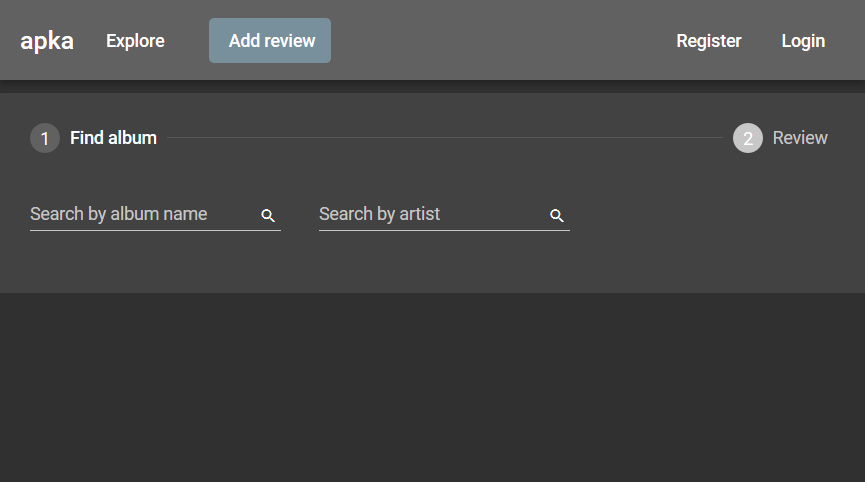
\includegraphics[height=200px]{rys05/gt-xs.png}
			 \caption{Menu nawigacji dla zwykłych ekranów}
			 \label{fig:gt-xs}
		\end{figure}

		\begin{figure}[ht]
			\centering
				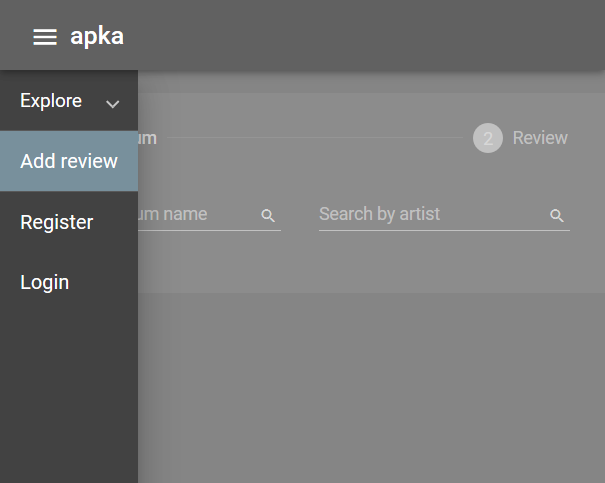
\includegraphics[height=200px]{rys05/xs.png}
			 \caption{Wysunięte manu nawigacji dla małych ekranów}
			 \label{fig:xs}
		\end{figure}

	\subsection{Motyw aplikacji}
		W aplikacji skorzystano z biblioteki \emph{Anuglar Material}, która oprócz gotowych, często używanych komponentów,
		ułatwia korzystanie z globalnego motywu kolorystycznego.
		Definiowanie kolorystyki odbywa się za pomoca \emph{mixin}, które określają kolory poszczególnych komponentów.
		Zaimplementowane zostały dwa motywy, choć dodanie kolejnego wiąże się jedynie ze zdefiniowaniem kolorystyki w jednym miejscu.
		Domyślny, ciemny motyw zdefiniowany został następująco:
		\begin{lstlisting}[label=lst:darkTheme]
			$dark-primary: mat-palette($mat-grey, 700, 300, 900);
			$dark-accent: mat-palette($mat-blue-grey, 400);
			$dark-warn: mat-palette($mat-red, 500);
			
			$dark-theme: mat-dark-theme($dark-primary, $dark-accent, $dark-warn);
		\end{lstlisting}
		Funkcja \verb|mat-palette| zwraca paletę kolorów: pierwszy argument określa bazową paletę koloru, a kolejne trzy odpowiednio domyślny, jasny i ciemniejszy odcień.
		Metoda \verb|mat-dark-theme| oraz analogiczna \verb|mat-light-theme| oprócz przekazanych palet kolorów definiują dodatkowo domyślne kolory tła.
		Na podstawie tych mixin-ów stworzone zostały dwa style css:
		\begin{lstlisting}			
			@mixin custom-components-theme($theme) {
				@include header-component-theme($theme);
				@include sidenav-component-theme($theme);
				@include album-grid-component-theme($theme);
				@include album-search-component-theme($theme);
			}
			
			.light-theme {
				@include angular-material-theme($light-theme);
				@include custom-components-theme($light-theme);
			}
			
			.dark-theme {
				@include angular-material-theme($dark-theme);
				@include custom-components-theme($dark-theme);
			}	
		\end{lstlisting}

		Aby wykorzystać kolory motywu we własnych komponentach (nie zawartych w \verb|angular-material-theme|),
		należy stworzyć nowy \emph{mixin}, który może pobierać ustawione kolory za pomocą funkcji \verb|map-get|.
		Przykładowy \emph{mixin}, który wykorzystuje tą metodę jest następujący:
		\begin{lstlisting}
			@mixin sidenav-component-theme($theme) {
				$primary: map-get($theme, primary);
				$accent: map-get($theme, accent);
			
				mat-sidenav {
					button, .mat-list-item {
						&.active {
							color: mat-color($accent, default-contrast);
							background-color: mat-color($accent);
			
							&:hover {
								background-color: mat-color($accent, darker);
							}
						}
					}
				}
			}			
		\end{lstlisting}

		Przełączanie pomiędzy globalnymi stylami odbywa się w głównym komponencie aplikacji \verb|app.component|,
		przedstawionym na listingu~\ref{lst:appComponent}, w pierwszej linijce.
		Odpowiednia klasa aktywowana jest na podstawie wartości \verb|theme| ustawień użytkownika.

\section{GraphQL API}
	Api stworzone zostało na platformie .Net Core 3.0.
	Wykorzystane zostały następujące technologie:
	\begin{description}
		\item[Hot Chocolate] --- platforma pozwalająca zbudować serwer GraphQL na infrastrukturze .NET.
			Umożliwia definiowanie schematu GraphQL zarówno za pomocą języka SDL (ang.\ \emph{Schema Definition Language}),
			jak i języka C\# poprzez podejście code-first. 
		\item[Autofac] --- biblioteka dostarczająca zaawansowany kontener służący do inwersji kontroli (IoC - \emph{Inversion of Control}).
			Pozwala na szczegółowe lub automatyczne definiowanie interfejsów i ich implementacji.
		\item[Entity Framework Core] --- narzędzie służące jako ORM (ang.\ \emph{Object-Relational Mapper}).
			Automatyzuje dostęp do bazy danych poprzez mapowanie encji bazodanowych na obiekty POCO (ang.\ \emph{Plain Old CLR Object}).
			Dodatkowo umożliwia generowanie bazy danych na podstawie modeli, tworząc migrację po każdej zmianie na istniejącej bazie.
	\end{description}

	\subsection{Warstwa Api}
		W tej warstwie skonfigurowany został serwer GraphQL.
		Zdecydowano sie definiować schemat metodą code-first, aby wykorzystać modele warstwy domenowej jako bazy typów.

		\subsubsection*{Generowanie typów}
			Biblioteka \emph{Hot Chocolate} umożliwia automatyczne generowanie typów z klas.
			Dodatkowo, w projekcie załączono opcjonalną funkcjonalność \emph{Nullable reference types} wprowadzoną w C\#8.0 i zaimplementowaną w .NET Core 3.0.
			Sprawia ona, że typy referencyjne domyślnie oznaczane są jako non-null, czyli nigdy nie będą równe null.
			Aby oznaczyć pole jako dopuszczające wartość null należy oznaczyć je znakiem zapytania.
			Jest to działanie analogiczne do typów wartościowych i pomaga zapobiegać nieobsłużonym wyjątkom \emph{Null Reference Exception}.
			W użytej wersji \emph{Hot Chocolate} (10.1.1), nie są one jednak interpretowane --- wszystkie typy referencyjne oznaczane są jako obowiązkowe pola.
			Biblioteka ta pozwala jednak na rozszerzanie domyślnych konwencji, co postanowiono wykorzystać do zaimplementowania automatycznego oznaczania typów referencyjnych.
			Skorzystano przy tym z biblioteki \emph{Namotion.Reflection}, która rozszerza refleksję o metody sprawdzające, czy w danym kontekście typ może przyjmować null, czy nie.
			W ten sposób powstała klasa \verb|TypeInspector|, wprowadzająca następujące modyfikacje do automatycznego generowania typów:
			\begin{itemize}
				\item klucze obce w modelach nie są tłumaczone na pola typów graphql, ponieważ wykorzystywane są jedynie wirtualne pola nawigacyjne (ang.\ \emph{navigation property}),
				\item pola z referencyjnymi typami są poprawnie oznaczane jako opcjonalne lub obowiązkowe.
			\end{itemize}

			Jeśli wymagana jest dodatkowa konfiguracja to tworzona jest funkcją \verb|Configure|.
			Dla typu \verb|AlbumType| nazwa pola \verb|MusicBrainzId| ustawiana jest na \verb|mbid|, gdyż pod taką nazwą pobierane jest z Api Last.fm:
			\begin{lstlisting}
				public class AlbumType : ObjectType<Album>
				{
					protected override void Configure(
						IObjectTypeDescriptor<Album> descriptor)
					{
						descriptor.Field(t => t.MusicBrainzId)
							.Type<StringType>()
							.Name("mbid");
					}
				}
			\end{lstlisting}

		\subsubsection*{Generowanie odpowiedzi}
			Klasa \verb|Query| zawiera metody, które zwracają odpowiednie wartości dla zapytań.
			Listing~\ref{lst:queryClr} przedstawia dwie takie metody.
			\verb|GetAlbum| to prosta metoda zwracająca album o danym id z repozytorium, którego implementacja znajduje się w warstwie Infrastructure.
			\verb|SearchArtists| wyszukuje artystów wykorzystując metodę \verb|Search|, która jako argument przyjmuje obiekt typu \emph{Expression<Func<T, bool>>}.
			\emph{Expression tree} w przeciwieństwie do delegatów typu \emph{Func<>} nie kompiluje się do IL (ang.\ \emph{Intermediate Language}),
			dzięki czemu Entity Framework może przetłumaczyć wyrażenie na zapytanie SQL.
			C\# automatycznie tłumaczy anonimowe funkcje lambda na wyrażenie, jednak nie wszystkie metody są tłumaczone.
			Z tego powodu podczas porównania nazwy artysty z zapytaniem na obu argumentach wykonywana jest funkcja \verb|ToLower()|,
			zamiast użycia \verb|StringComparison.OrdinalIgnoreCase|.

			\begin{lstlisting}[label=lst:queryClr, caption=Fragment klasy Query, float]
				private readonly IRepository _repository;
		
				public Query(IRepository repository)
				{
					_repository = repository;
				}

				public Album? GetAlbum(Guid id) => _repository.GetById<Album>(id);

				public IEnumerable<Artist> SearchArtists(string? mbid, string name)
				{
					List<Artist>? results = null;
					if (!string.IsNullOrEmpty(mbid))
						results = _repository.List<Artist>(artist =>
							artist.MusicBrainzId == mbid);
		
					return results?.Count > 0
						? results
						: _repository.Search<Artist>(artist =>
							artist.Name.ToLower().Contains(name.ToLower()));
				}
			\end{lstlisting}

		\subsubsection*{Middleware}
			Podczas przetwarzania niektórych zapytań wymagane są dodatkowe akcje.
			Wykorzystywane są do tego \emph{middleware}.
			Przykładowym, wbudowanym middleware jest dyrektywa \emph{authorize}.
			Sprawdza ona, czy zalogowany użytkownik posiada prawa do wywołania odpowiedniego pola wykorzystując wbudowany system Identity.
			
			W projekcie stworzony został nowy middleware (Listing~\ref{lst:middleware}), który dodaje do bazy Api zalogowanego użytkownika, aby można było powiązać z nim dodawane occeny.
			Serwis pobiera id zalogowanego użytkownika z kontekstu, a następnie sprawdza, czy taki użytkownik już istnieje.
			Jeśli nie, to wykorzystuje \verb|OpenIdService| (opisany w rozdziale~\ref{sec:oidApi}),
			aby pobrać nazwę użytkownika z serwera uwierzytelniającego.
			Następnie dane te zapisuje w bazie za pomocą repozytorium.
			Na końcu przekazuje zapytanie do dalszego przetwarzania poprzez \verb|_next(context)|.
			Tak napisaną klasę można zarejestrować jako middleware podczas konfiguracji dowolnego typu, np.\ mutacji:
			\begin{lstlisting}
				descriptor.Field(t => t.AddRating(default!, default!))
					.Use<RecordUserMiddleware>()
					.Argument("rating", a => a.Type<NonNullType<RatingInputType>>())
					.Type<NonNullType<AlbumType>>();
			\end{lstlisting}

			\begin{lstlisting}[label=lst:middleware, caption=Middleware zapisujące użytkowników, float]
				public class RecordUserMiddleware
				{
					private readonly FieldDelegate _next;
					private readonly OpenIdService _openIdService;
			
					public RecordUserMiddleware(
						FieldDelegate next,
						OpenIdService openIdService)
					{
						_next = next;
						_openIdService = openIdService;
					}
			
					public async Task InvokeAsync(
						IMiddlewareContext context,
						IRepository repository,
						IHttpContextAccessor httpContextAccessor)
					{
						var id = httpContextAccessor.HttpContext.User
							.FindFirstValue(ClaimTypes.NameIdentifier);
			
						var user = repository.GetById<User>(new Guid(id));
			
						if (user == null)
						{
							var accessToken = await httpContextAccessor.HttpContext
								.GetTokenAsync("access_token");
							var userInfo = await _openIdService.GetUserInfo(accessToken);
			
							repository.Add(new User
							{
								Id = userInfo.Sub,
								Username = userInfo.Name
							});
						}
			
						await _next(context);
					}
				}
			\end{lstlisting}

	\subsection{Warstwa domenowa}
		Warstwa domenowa zawiera logikę biznesową aplikacji: encje, serwisy i interfejsy.
		Interfejsy definiują abstrakcje operacji, które wykonywane będą w warstwie infrastruktury.
		Są to dostęp do systemu plików, połączenie z bazą danych czy zapytania HTTP.

		Encje posiadają zadeklarowane zarówno klucze obce, jak i wirtualne ścieżki.
		Wirtualne ścieżki wykorzystywane są do zagnieżdżania zapytań graphql, natomiast klucze obce podczas dodawania nowych wpisów do bazy.
		W projekcie zaimplementowano wzorzec projektowy \emph{Repository}.
		Stworzono w tym celu generyczny interfejs definiujący repozytorium:
		\begin{lstlisting}
			public interface IRepository
			{
				T? GetById<T>(Guid id) where T : BaseEntity;
				List<T> List<T>() where T : BaseEntity;
				List<T> List<T>(Expression<Func<T, bool>> filter) where T : BaseEntity;
				T Add<T>(T entity) where T : BaseEntity;
				T Update<T>(T entity) where T : BaseEntity;
				void Delete<T>(T entity) where T : BaseEntity;
			}
		\end{lstlisting}
		Przyjmowany typ \verb|T| musi dziedziczyć po \verb|BaseEntity|, co zapewnia obecność pola \verb|Id| typu Guid.
		Implementacja repozytorum opisana została w następnym rozdziale.

	\subsection{Warstwa infrastruktury}
		W tej warstwie znajdują się implementacje dostępu do danych oraz rejestracja zależności aplikacji.

		\subsubsection*{Dostęp do danych}
			Jest to jedyna warstwa aplikacji, która deklaruje jako zależność bibliotekę \emph{Entity Framework Core}.
			Klasa \verb|EfRepository| (Listing~\ref{lst:repository}) implementuje interfejs zdefiniowany w warstwie Core wykorzystując EF Core.
			Ona również jest generyczna, ponieważ operacje na wszystkich encjach są analogiczne.
			Bardziej skomplikowane zapytania wymusiły by stworzenie nowego interfejsu, lub wyizolowanie funkcji \verb|_dbContext.SaveChanges| jako osobnej metody.
			Wtedy możliwe było by przeprowadzenie wielu operacji w ramach tej samej transakcji.
			W obecnej implementaji każde zapytanie modyfikujące bazę zamyka transakcję.
			W tej klasie umieszczane są również inne transformacje zapytań wykonywane za każdym razem,
			np.\ pomijanie wpisów, które oznaczone zostały jako nieaktywne (ang.\ \emph{soft delete}).

			\begin{lstlisting}[label=lst:repository, caption=Implementacja repozytorium, float]
				public class EfRepository : IRepository
				{
					private readonly AppDbContext _dbContext;
			
					public EfRepository(AppDbContext dbContext)
					{
						_dbContext = dbContext;
					}
					public T? GetById<T>(Guid id) where T : BaseEntity
					{
						return _dbContext.Set<T>().SingleOrDefault(e => e.Id == id);
					}
					public List<T> List<T>() where T : BaseEntity
					{
						return _dbContext.Set<T>().ToList();
					}
					public List<T> List<T>(Expression<Func<T, bool>> filter)
							where T : BaseEntity
					{
						return _dbContext.Set<T>().Where(filter).ToList();
					}
					public T Add<T>(T entity) where T : BaseEntity
					{
						_dbContext.Set<T>().Add(entity);
						_dbContext.SaveChanges();
			
						return entity;
					}
					public T Update<T>(T entity) where T : BaseEntity
					{
						_dbContext.Entry(entity).State = EntityState.Modified;
						_dbContext.SaveChanges();
			
						return entity;
					}
					public void Delete<T>(T entity) where T : BaseEntity
					{
						_dbContext.Set<T>().Remove(entity);
						_dbContext.SaveChanges();
					}
				}
			\end{lstlisting}
			
			Do tłumaczenia zapytań na język SQL kompatybilny z bazą PostgreSQL wykorzystano bibliotekę \emph{Npgsql}.
			Przykładowo, wywołanie z listingu~\ref{lst:queryClr} wyszukujące po nazwie artysty zostanie przetłymaczone na zapytanie wykorzystuje motodę \verb|STRPOS|,
			znajdującą pozycję ciągu znaków w tekście, oraz \verb|LOWER|, zmieniającą znaki w tekście na małe litery:
			\begin{lstlisting}
				Executing DbCommand [Parameters=[@__ToLower_0='name']
				SELECT a."Id", a."MusicBrainzId", a."Name"
				FROM "Artists" AS a
				WHERE STRPOS(LOWER(a."Name"), @__ToLower_0) > 0
			\end{lstlisting}
			
			Aby uniknąć dodawania referencji do bibliotek związanych z dostępem do bazy, rejestracja DbContext również odbywa się w tej warstwie.
			Stworzono w tym celu metodę rozszerzającą,
			która rozszerza klasę IServiceCollection o metodę AddDbContext przyjmującą connection string do bazy.
			\begin{lstlisting}
				public static void AddDbContext(
					this IServiceCollection services, string connectionString) =>
					services.AddDbContext<AppDbContext>(options =>
					{
						options.UseLazyLoadingProxies();
						options.UseNpgsql(connectionString);
					});
			\end{lstlisting}
			Metoda ta rejestruje kontekst bazy wykorzystując funkcję \verb|UseNpgsql| biblioteki \emph{Npgsql}.
			Dodatkowo, w opcjach użyto metody \verb|UseLazyLoadingProxies|.
			Jest to rozszerzenie zawarte w bibliotece \emph{Microsoft.EntityFrameworkCore.Proxies},
			które pozwala na późne ładowanie (ang.\ \emph{lazy loading}) pokrewnych encji.
			Dzięki temu możliwe jest wykonywanie zapytań o dowolnej głębokości zagnieżdżenia bez jawnej deklaracji, które tablice mają zostać załadowane.
			
			Należy jednak mieć na uwadze, że GraphQL sam w sobie nie stanowi rozwiązania problemu N+1.
			Jest to problem wynikający z ładowania pokrewnych wpisów.
			Dla jednego zapytania wykonywane jest kolejnych N zapytań, po jednym dla każdej relacji, stąd N+1.
			Przykładowo, dla zapytania zawierającego podwójne zagnieżdżenie, gdzie dla każdego albumu zwracane są piosenki:
			\begin{lstlisting}
				query getart {
					artist(id: "a0000000-0000-0000-0000-000000000001") {
						id
						name
						albums {
							id
							title
							songs {
								id
								title
							}
						}
					}
				}
			\end{lstlisting}
			wykonywane są następujące komendy SQL:
			\begin{lstlisting}
				[Parameters=[@__id_0='a0000000-0000-0000-0000-000000000001']
				SELECT a."Id", a."MusicBrainzId", a."Name"
				FROM "Artists" AS a
				WHERE (a."Id" = @__id_0) AND (@__id_0 IS NOT NULL)
				LIMIT 2

				[Parameters=[@__p_0='a0000000-0000-0000-0000-000000000001']
				SELECT a."Id", a."AlbumArtistId", a."AverageRating"
					a."CoverSrc", a."MusicBrainzId", a."ReleaseDate", a."Title"
				FROM "Albums" AS a
				WHERE (a."AlbumArtistId" = @__p_0) AND (@__p_0 IS NOT NULL)

				[Parameters=[@__p_0='b0000000-0000-0000-0000-000000000000']
				SELECT s."Id", s."AlbumId", s."ArtistId", s."Length"
					s."MusicBrainzId", s."Title", s."TrackNumber"
				FROM "Songs" AS s
				WHERE (s."AlbumId" = @__p_0) AND (@__p_0 IS NOT NULL)

				[...]

				[Parameters=[@__p_0='b0000000-0000-0000-0000-000000000009']
				SELECT s."Id", s."AlbumId", s."ArtistId", s."Length"
					s."MusicBrainzId", s."Title", s."TrackNumber"
				FROM "Songs" AS s
				WHERE (s."AlbumId" = @__p_0) AND (@__p_0 IS NOT NULL)
			\end{lstlisting}
			W pierwszej kolejności wczytywane są dane artysty oraz jego albumów (pierwsze dwa zapytania).
			Następnie dla każdego z tych albumów ładowane są piosenki --- kolejnych 10 zapytań do bazy.
			Jest to typowy problem ładowania danych, który powstaje podczas późnego ładowania powiązanych wpisów.
			Jednym z możliwych rozwiązań jest wczesne ładowanie, czyli zadeklarowanie, które relacje mają zostać załadowane jeszcze przed wykonaniem zapytania do bazy.
			Jednak w związku z tym, że klient korzystający z GraphQL może zarządać dowolną relację, nie ma możliwości statycznego zadeklarowania, które tablice mają zostać załadowane.
			Potrzebne jest zatem dynamiczne rozwiązanie, które będzie interpretować zapytania i dołączać odpowiednie relacje bazy danych.
			Można również zaimplementować \emph{data loader} --- narzędzie, które wysyła zapytania w partiach oraz wprowadza dodatkową warstwę cache.

		\subsubsection*{Rejestracja zależności}
			Rejestracja zależności odbywa się przy pomocy narzędzia \emph{Autofac}.
			Metoda \verb|InitializeApi|, wywoływana na końcu metody \verb|ConfigureServices| klasy \verb|Startup| warstwy Api,
			W pierwszej kolejności w kontenerze Autofac rejestrowane są wszystkie serwisy z projektów Core oraz Infrastructure.
			Funkcja \verb|RegisterAssemblyTypes| skanuje całe assembly (skompilowany projekt) i wyszukuje serwisy utworzone zgodnie z przyjętymi konwencjami.
			Następnie do kontenera przekazywane są wszystkie dotychczas zarejestrowane serwisy,
			po czym skanownane jest assembly warstwy Api, przekazane podczas wywołania konfiguracji:
			\begin{lstlisting}
				ContainerSetup.InitializeApi(Assembly.GetExecutingAssembly(), services);
			\end{lstlisting}

			\begin{lstlisting}[label=lst:autofac, caption=Rejestracja zależności wykorzystująca Autofac, float]
				public static IServiceProvider InitializeApi(
					Assembly webAssembly, IServiceCollection services) =>
					new AutofacServiceProvider(BaseAutofacInitialization(setupAction =>
					{
						setupAction.Populate(services);
						setupAction.RegisterAssemblyTypes(webAssembly)
							.AsImplementedInterfaces();
					}));
	
				public static IContainer BaseAutofacInitialization(
					Action<ContainerBuilder>? setupAction)
				{
					var builder = new ContainerBuilder();
		
					var coreAssembly = Assembly.GetAssembly(typeof(BaseEntity));
					var infrastructureAssembly = Assembly.GetAssembly(typeof(EfRepository));
					builder.RegisterAssemblyTypes(coreAssembly, infrastructureAssembly)
						.AsImplementedInterfaces();
		
					setupAction?.Invoke(builder);
					return builder.Build();
				}
			\end{lstlisting}
	
\section{Serwis uwierzytelniający}
	Serwis również stworzony został na platformie Microsoftu.
	Do zaimplementowania głównej funkcjonalności wykorzystano następujące biblioteki:
	\begin{description}
		\item[IdentityServer4] 
		\item[AspNetCore.Identity] 
	\end{description}

	Zarówno rejestracja jak i logowanie wykorzystują widoki dostarczone przez Identity.
	Podczas wykonywania tych akcji użytkownik zostaje przekierowany na serwer Auth przy pomocy odwróconego proxy.

	\subsection{Konfiguracja}
		Na serwerze zarejestrowany został jeden klient, \verb|angular_spa|, z którego korzystać będą użytkownicy.
		Poniżej opisane zostały najważniejsze opcje:
		\begin{description}
			\item[ClientId] Id klienta musi być takie same zarówno po stronie serwera jak i klienta
			\item[AllowedGrantTypes] dozwolone tryby uwierzytelniania. Dozwolono jedynie tryb wykorzystujący kod autoryzacji
			\item[RequirePkce] wymagane użycie kodu PKCE
			\item[AllowedScopes] dozwolone zakresy informacji o użytkowniku, o które może poprosić klient
			\item[RedirectUris] adresy, na które może przekierować aplikacja
		\end{description}
		\begin{lstlisting}[label=lst:openIdSrv, caption=Konfiguracja OpenId po stronie serwera, float]
			ClientId = "angular_spa",
			ClientName = "Angular SPA",
			RequireConsent = false,
			AllowedGrantTypes = GrantTypes.Code,
			RequirePkce = true,
			RequireClientSecret = false,
			AllowedScopes = {"openid", "profile", "email"},
			RedirectUris = {
				"http://localhost/login-callback",
				"http://localhost/register-callback",
				"http://localhost/silent-refresh"},
			PostLogoutRedirectUris = {"http://localhost/"},
			AllowedCorsOrigins = {"http://localhost"},
			AllowAccessTokensViaBrowser = true,
			AccessTokenLifetime = 3600
		\end{lstlisting}

		\begin{lstlisting}[label=lst:openIdSpa, caption=Konfiguracja OpenId po stronie Spa, float]
			authority: environment.authServerUri,
			client_id: 'angular_spa',
			response_type: 'code',
			scope: 'openid profile email api.read',
			filterProtocolClaims: true,
			loadUserInfo: true,
			automaticSilentRenew: true,
			redirect_uri: `${environment.thisUri}/login-callback`,
			post_logout_redirect_uri: `${environment.thisUri}/`,
			silent_redirect_uri: `${environment.thisUri}/silent-refresh`
		\end{lstlisting}

	\subsection{Rejestracja}
		Podczas rejestracji użytkownik podaje login i hasło.
		Na podstawie tych danych tworzony jest nowe konto i zapisywane jest w bazie danych przez pomocniczy obiekt klasy \verb|UserManager|,
		jak ukazano na listingu~\ref{lst:register}.
		Następnie użytkownik zostaje przekierowany z powrotem na serwis SPA.

		\begin{lstlisting}[label=lst:register, caption=Fragment kodu rejestacji, float]
			var user = new IdentityUser {UserName = Input.Email, Email = Input.Email};
			var result = await _userManager.CreateAsync(user, Input.Password);
			if (result.Succeeded)
			{
				await _signInManager.SignInAsync(user, isPersistent: false);
				return Redirect(returnUrl);
			}
		\end{lstlisting}

	\subsection{Logowanie}
		Logowanie odbywa się wykorzystując protokół OpenID z kodem autoryzacji i PKCE opisanym w rozdziale~\ref{sec:openid}.
		W pierwszym kroku klient pobiera konfigurację serwera dostępną pod ustandaryzowanym adresem \verb|/.well-known/openid-configuraion|.
		Jest to plik typu JSON definiujący pełną konfigurację serwisu uwierzytelniającego oraz adresy punktów dostępowych.
		Na podstawie tej konfiguracji klient wykonuje zapytanie logowania pod adres \verb|/connect/authorize| z następującymi parametrami:
		\begin{lstlisting}
			client_id: angular_spa
			redirect_uri: http://localhost/login-callback
			response_type: code
			scope: openid profile email api.read
			state: 785f3544ba2a4df896290ccf5fedd51b
			code_challenge: 9e5S4as5foL7Y4ye6JQfl3Uuyd9HzmYli4Y732RLqys
			code_challenge_method: S256
			response_mode: query
		\end{lstlisting}
		Parametr \verb|code_challenge| to wartość \verb|code_verifier| zmodyfikowana przez funkcję \verb|S256|.
		Funkcja ta zdefiniowana jest w punkcie 4.2 RFC 7636~\cite{PKCE}:
		\begin{lstlisting}
			code_challenge = BASE64URL-ENCODE(SHA256(ASCII(code_verifier)))
		\end{lstlisting}
		Zapytanie to skutkuje przekierowaniem na stronę logowania \verb|/Login|.
		Po podaniu prawidłowych danych użytkownik przekierowywany jest z powrotem na główną stronę, a w pasku adresu widoczne są następujące parametry:
		\begin{lstlisting}
			code: stR57rgpV11RCd09AMn2PBuxKh0tb3CoW_V9ULehChg
			scope: openid profile email api.read
			state: 785f3544ba2a4df896290ccf5fedd51b
			session_state: [...]
		\end{lstlisting}
		Następnie w tle wykonywane jest zapytaniepod adresem \verb|/connect/token|  pobierające tokeny JWT:
		\begin{lstlisting}
			client_id: angular_spa
			code: stR57rgpV11RCd09AMn2PBuxKh0tb3CoW_V9ULehChg
			redirect_uri: http://localhost/login-callback
			code_verifier: 5d797a22803645fc870b1f1d6c9e5dfc...
			grant_type: authorization_code
		\end{lstlisting}
		Aplikacja precyzuje tryb uwierzytelaniania na \verb|authorization_code| i wysyła otrzymany przed chwilą kod autoryzacji.
		Przesyłany jest również \verb|code_verifier| --- klucz, który wcześniej został przesłany w zmodyfikowanej wersji.
		Serwer przekształca \verb|code_verifier| sprecyzowaną wczesniej funkcją \verb|code_challenge_method| i porównuje z \verb|code_challenge|.
		Jeśli są sobie równe, w odpowiedzi aplikacja otrzymuje zarówno \verb|id_token|, jak i \verb|access_token|:
		\begin{lstlisting}
			id_token: [...]
			access_token: [...]
			expires_in: 3600
			token_type: Bearer
			scope: openid profile email api.read
		\end{lstlisting}
		Uzyskany token zostaje użyty do pobrania informacji o użytkowniku.
		Służy do tego punkt połączeniowy \verb|/connect/userinfo|.
		Przesyłany jest nie jako parametr, lecz jako nagłówek HTTP \verb|Authorization: Bearer [access_token]|.
		W odpowiedzi serwer zwraca dane użytkownika identyfikującym się tym tokenem:
		\begin{lstlisting}
			sub: 0d6dfb71-745e-47c2-81f0-c9649bf0a2b2
			preferred_username: a@a.a
			name: a@a.a
			email: a@a.a
			email_verified: false
		\end{lstlisting}
		Ten sam token przekazywany jest podczas zapytań do serwisu API.

	\subsection{Autoryzacja dostępu do API}\label{sec:oidApi}
		Serwis Apollo po stronie SPA przekazuje w nagłówku autoryzacji token dostępowy, jak ukazano na listingu~\ref{lst:apolloSettings}.
		Do walidacji tokena po stronie API użyta została wbudowana w .NET Core metoda \verb|AddJwtBearer|:
		\begin{lstlisting}
			services.AddAuthentication("Bearer").AddJwtBearer("Bearer", options =>
			{
				options.Authority = "http://authServer";
				options.Audience = "reServer";
				options.RequireHttpsMetadata = false;
				options.TokenValidationParameters.ValidIssuer = "http://auth";
				options.SaveToken = true;
			});
		\end{lstlisting}
		W opcjach podano parametry służące do walidacji tokena:
		\begin{description}
			\item[Authority] to adres serwera, który wystawił token
			\item[Audience] to identyfikator serwera zawierającego dane, do których dostęp daje \verb|access_token|
			\item[RequireHttpsMetadata] szyfrowane połączenie nie jest wymagane, ponieważ zapytania do serwisu Auth nie wychodzą poza wewnętrzną sieć dockerową
			\item[TokenValidationParameters.ValidIssuer] ustawione na taką samą wartość jak po stronie serwisu Auth.
				Jest to wymagane, ponieważ serwis Auth przyjmuje zapytania zarówno z zewnątrz przez odwrócone proxy, jak i z wewnętrznej sieci dockerowej.
		\end{description}

		Tak ustawiony middleware rejestrowane jest w funkcji Configure, która definiuje kolejność obsługiwania zapytań HTTP:
		\begin{lstlisting}
			app.UseAuthentication();
			app.UseAuthorization();
		\end{lstlisting}
		Dzięki temu dane uwierzytelnionego użytkownika dostępne są w \verb|HttpContext.User| i mogą zostać wykorzystane w innych warstwach aplikacji, jak ukazano na listingu~\ref{lst:middleware}.
		Klasa ta wykorzystuje serwis \verb|OpenIdService| --- skonfigurowany klient HTTP, który łączy się z serwisem Auth (Listing~\ref{lst:openIdService}).
		Dane pobierane są z adrestu \verb|/connect/userinfo| przesyłając token w nagłówku \verb|Authorization|.
		Odpowiedź z serwera serializowana jest do zdefiniowanej klasy \verb|UserInfo|.
		\begin{lstlisting}[label=lst:openIdService, caption=Serwis HTTP pobierający dane użytkownika, float]
			public class OpenIdService
			{
				public HttpClient Client { get; }
		
				public OpenIdService(HttpClient client)
				{
					client.BaseAddress = new Uri("http://authServer/connect/");
					Client = client;
				}
		
				public async Task<UserInfo> GetUserInfo(string accessToken)
				{
					Client.DefaultRequestHeaders.Authorization
						= new AuthenticationHeaderValue("Bearer", accessToken);
					var response = await Client.GetAsync("userinfo");
					response.EnsureSuccessStatusCode();
		
					using var responseStream = await response.Content.ReadAsStreamAsync();
					return await JsonSerializer.DeserializeAsync<UserInfo>(responseStream);
				}
			}
		\end{lstlisting}

\section{Baza danych}
	



\section{Odwrócone proxy}